% =================================================================
% SUPPLEMENTARY MATERIAL (STANDALONE DOCUMENT)
% =================================================================
\documentclass[11pt,a4paper]{article}
\usepackage{iftex}
\ifXeTeX\else
  \PackageError{paper-template}{XeLaTeX is required}{Run xelatex; fontspec requires XeLaTeX.}
\fi
\usepackage{fontspec}
\IfFontExistsTF{Liberation Serif}{\setmainfont{Liberation Serif}}{\setmainfont{Times New Roman}}
\usepackage{graphicx}
\usepackage{amsmath,amssymb,amsfonts}
\usepackage[a4paper, margin=1in]{geometry}
\usepackage{setspace}
\setstretch{1.12}
\usepackage{booktabs}
\usepackage{microtype}
\usepackage{xcolor}
\usepackage{array}
\usepackage{tabularx}
\usepackage{multirow}
\usepackage{xurl}
\usepackage[hidelinks,unicode=true]{hyperref}
\urlstyle{same}
\usepackage{caption}
\usepackage{placeins}
\captionsetup{
  font=small,
  labelfont=bf,
  textfont=normalfont,
  labelsep=period,
  justification=justified,
  singlelinecheck=true,
  skip=6pt
}

\renewcommand{\thesection}{S\arabic{section}}
\renewcommand{\thetable}{S\arabic{table}}
\renewcommand{\thefigure}{S\arabic{figure}}
\renewcommand{\theequation}{S\arabic{equation}}

\usepackage{fancyhdr}
\setlength{\headheight}{14pt}
\pagestyle{fancy}
\fancyhf{}
\fancyhead[L]{\small Supplementary Material --- NORS Pathogen Hospitalization Orderings}
\fancyhead[R]{\small\thepage}
\renewcommand{\headrulewidth}{0.4pt}
\fancypagestyle{plain}{
  \fancyhf{}
  \fancyfoot[C]{\small\thepage}
  \renewcommand{\headrulewidth}{0pt}
}

\usepackage{newunicodechar}
\newunicodechar{δ}{\ensuremath{\delta}}

\title{\textbf{Supplementary Material}\\[0.4em]
\large Hospitalization Orderings among Six Pathogen Groups in Foodborne Outbreaks with Incompletely Recorded Outcomes, United States, 2009--2023}
\author{Apevon Science}
\date{\today}

\begin{document}
\maketitle
\normalfont\mdseries

\section{Study Population, Settings and Reference Weights}\label{sec:s-population}

Of 11,358 foodborne outbreaks reported to NORS for 2009--2023, 4,133 met the primary eligibility criteria: 3,908 listed a single confirmed etiology entry and 225 listed multiple serotype or genotype entries mapping to a single study group with at least one confirmed entry. Confirmed norovirus outbreaks lacking genogroup specification (304 outbreaks) and outbreaks combining entries across study groups or with non-study agents (300 outbreaks; 104 containing at least one confirmed study-group entry) were excluded because outcome counts cannot be attributed to a single study group. Across the 4,133 eligible outbreaks, record auditing identified 3,976 complete and consistent records, 52 records with blank $K_i$, 28 with blank $H_i$ and $K_i = 0$, 23 with blank $H_i$ and $K_i > 0$, and 54 with both fields blank, with zero count contradictions (Table~\ref{tab:audit}). After retaining all 157 incomplete records under logical bounds, 19.4\% of eligible cases had unrecorded hospitalization status.

Raw NORS food-preparation setting tokens were harmonized into seven mutually exclusive categories: \textit{Restaurant} (sit-down, fast-food, buffet, other restaurant, food truck/street vendor), \textit{Catering or banquet} (caterer, banquet facility, event space), \textit{Private home} (private home/residence, single-family or multi-unit housing), \textit{Institution} (school/college/university, long-term care/nursing home, correctional facility, hospital, other healthcare facility, child daycare/preschool, camp, office/workplace, soup kitchen), \textit{Other} (grocery/bakery/deli, festival/fair, religious facility, farm/dairy, hotel/motel, ship/boat, park, campground, commissary, other), \textit{Multiple} (entries spanning two or more named categories after ignoring ``Unknown'' tokens when paired with a known setting) and \textit{Unknown} (only ``Unknown'' or blank).

Crossing the seven setting categories with three five-year periods (2009--2013, 2014--2018 and 2019--2023) yielded 21 candidate cells, of which 12 contained at least 3 outbreaks for all six groups. Their pooled-case reference weights $w_s$ were: restaurant in 2009--2013 (16.1\%), 2014--2018 (17.7\%) and 2019--2023 (9.6\%); catering or banquet in 2014--2018 (8.6\%); private home in 2009--2013 (5.8\%) and 2014--2018 (4.2\%); institution in 2009--2013 (5.3\%) and 2014--2018 (6.5\%); other in 2009--2013 (5.8\%) and 2014--2018 (5.4\%); multiple in 2014--2018 (7.5\%); and unknown in 2009--2013 (7.5\%). No cell in 2019--2023 outside restaurants met the 3-outbreak support requirement across all six groups. Group-specific retention is detailed in Table~\ref{tab:retention} and Figure~\ref{fig:s-retention}.

\section{Critical Deviations, Stacked M-Estimation Influence Functions and VoI Protocol}\label{sec:s-deltastar}

\subsection*{Exact Piecewise-Linear Solution for $\delta^{*}_{hl}$}
For a pair ordered at $\delta = 0$ as $\theta_h(0) > \theta_l(0)$, the gap function
\begin{equation}
  g(\delta) = L_h(\delta) - U_l(\delta)
  = \sum_s w_s \frac{H_{hs} + M_{hs}\max(0,\, p_{hs} - \delta)}{C_{hs}}
  - \sum_s w_s \frac{H_{ls} + M_{ls}\min(1,\, p_{ls} + \delta)}{C_{ls}}
  \label{eq:s-gap}
\end{equation}
is continuous, monotonically non-increasing on $[0, 1]$ and piecewise linear with breakpoints at $\delta \in \{p_{hs}\}_s \cup \{1 - p_{ls}\}_s$ inside $(0, 1)$. When $g(1) > 0$, the ordering holds under worst-case bounds ($\delta^{*}_{hl} = \infty$). Otherwise, $\delta^{*}_{hl}$ was computed analytically by evaluating $g$ across sorted breakpoints and linearly interpolating within the unique interval $[\delta_k, \delta_{k+1}]$ where $g(\delta_k) > 0 \ge g(\delta_{k+1})$. Bisection agreed within $1.4 \times 10^{-14}$ points.

\subsection*{Closed-Form Influence Functions under Coupled Reference Weights}
Let $C_{\cdot} = \sum_{k=1}^{G}\sum_{t=1}^{K} C_{kt}$ denote total retained cases across the common support so that $w_t = C_{\cdot t}/C_{\cdot}$. For an arbitrary group $j$ and worst-case ratio $r^{L}_{jt} = H_{jt}/C_{jt}$ with standardized lower bound $\bar{L}_j = \sum_t w_t r^{L}_{jt}$, an outbreak $i$ in stratum $(k, s)$ perturbs $\bar{L}_j$ through two channels: (i) the shared reference-weight channel present for every $j \in \{1,\dots,G\}$, and (ii) the cell-rate channel present when $k = j$. Differentiating $\bar{L}_j(\mu)$ with respect to outbreak counts $(C_i, H_i, M_i)$ in $(k, s)$ gives the outbreak-level influence function:
\begin{equation}
  \psi^{L}_{j,i} = \frac{r^{L}_{js} - \bar{L}_j}{C_{\cdot}}(C_i - \bar{C}_{ks})
  + \mathbf{1}\{k = j\}\, \frac{w_s}{C_{js}} \left[(H_i - \bar{H}_{js}) - r^{L}_{js}(C_i - \bar{C}_{js})\right],
  \label{eq:s-if}
\end{equation}
with analogous expression $\psi^{U}_{j,i}$ replacing $H_i$ by $H_i + M_i$ and $r^{L}_{js}$ by $r^{U}_{js} = (H_{js} + M_{js})/C_{js}$. Writing $\psi_i = (\psi^{L}_{1,i},\dots,\psi^{L}_{G,i}, \psi^{U}_{1,i},\dots,\psi^{U}_{G,i})^{\top}$, summing $\frac{n_{ks}}{n_{ks}-1} \sum_{i \in (k,s)} \psi_i \psi_i^{\top}$ over all $(k,s)$ strata reproduces the central-difference stacked M-estimator sandwich covariance $\widehat{V}(1)$ to machine precision ($1.40 \times 10^{-12}$; Table~\ref{tab:cluster_diag}). For the 2,000-replicate bootstrap (seeded per replicate with seed pair \texttt{[20261125, b]}), if any resampled cell lacked recorded counts ($K_{\text{rec}} = 0$), that cell retained its worst-case bounds at all $\delta$, the $\delta = 0$ ordering direction was taken from the interval midpoint, and $\delta^{*}$ was set to $0$ whenever $g(0) \le 0$.

\subsection*{Retrospective Masking Protocol}
From the 3,176 common-support outbreaks, all 2,414 outbreaks with complete hospitalization records ($U_i = 0$; 45,249 cases) formed the ground-truth cohort. In each of 200 Monte Carlo trials (seed 20261125), outbreaks were masked independently with empirical cell-group incomplete probabilities bounded to $[0.12, 0.45]$, ensuring at least one unmasked outbreak per $(g, s)$ cell. Masked outbreaks were ranked by each of the four allocation rules using only the masked state, and outcomes were revealed sequentially up to follow-up budgets $B \in \{250, 500, 1000, 1500, 2000, 3500, 5000\}$ cases (Table~\ref{tab:voi_masking}).

\section{Supplementary Tables and Figures}\label{sec:s-tables}

% Table order S1..S7 and Figures S1..S3 matching main text citations:
% S1: table_5_audit
% S2: table_4_retention
% S3: table_3_robustness
% S4: table_6_bootstrap
% S5: table_9_cluster_diagnostics
% S6: table_7_width_decomposition
% S7: table_10_voi_masking

\begin{table}[!tbp]
\centering
\scriptsize
\setlength{\tabcolsep}{3pt}
\renewcommand{\arraystretch}{1.12}
\caption{Record audit of outbreak outcome fields (C reported cases, H hospitalized, K cases with known hospitalization status), with category counts and handling. No record had a count contradiction.}
\label{tab:audit}
\begin{tabular}{>{\raggedright\arraybackslash}p{2.1cm}>{\raggedleft\arraybackslash}p{1.4cm}>{\raggedleft\arraybackslash}p{1.1cm}>{\raggedleft\arraybackslash}p{0.92cm}>{\raggedleft\arraybackslash}p{0.92cm}>{\raggedleft\arraybackslash}p{0.92cm}>{\raggedleft\arraybackslash}p{0.92cm}>{\raggedleft\arraybackslash}p{0.92cm}>{\raggedleft\arraybackslash}p{0.92cm}>{\raggedright\arraybackslash}p{3.4cm}}
\toprule
Audit category & Outbreaks & Cases & SAL & STEC & CAMP & CPERF & NoV GI & NoV GII & Handling \\
\midrule
Complete and consistent & 3,976 & 95,781 & 1,689 & 369 & 292 & 180 & 285 & 1,161 & as recorded (K = 0 means all status unrecorded) \\
K blank & 52 & 2,337 & 26 & 6 & 0 & 2 & 3 & 15 & K set to H; remaining cases unrecorded \\
H blank, K = 0 & 28 & 978 & 11 & 3 & 2 & 2 & 1 & 9 & H = 0 implied by H $\leq$ K = 0; all cases unrecorded \\
H blank, K $>$ 0 & 23 & 321 & 1 & 1 & 0 & 1 & 5 & 15 & all cases treated as unrecorded \\
H and K blank & 54 & 3,623 & 31 & 9 & 2 & 3 & 3 & 6 & all cases treated as unrecorded \\
Ambiguous etiology & 408 & 12,220 & -- & -- & -- & -- & -- & -- & excluded (outcome not attributable to one group) \\
\bottomrule
\end{tabular}
\par\smallskip\parbox{0.97\linewidth}{\footnotesize Ambiguous etiology denotes confirmed entries of a study group together with entries of another group, or norovirus without genogroup; these outbreaks are not assigned to a group (--).}
\end{table}

\begin{table}[!tbp]
\centering
\scriptsize
\setlength{\tabcolsep}{3pt}
\renewcommand{\arraystretch}{1.12}
\caption{Common-support retention by pathogen group, with eligible and retained outbreaks and cases, the settings and periods losing most cases, and crude (unstandardized) proportions before and after the restriction.}
\label{tab:retention}
\begin{tabular}{>{\raggedright\arraybackslash}p{1.75cm}>{\raggedleft\arraybackslash}p{1.4cm}>{\raggedleft\arraybackslash}p{1.05cm}>{\raggedleft\arraybackslash}p{1.45cm}>{\raggedleft\arraybackslash}p{1.45cm}>{\raggedright\arraybackslash}p{1.85cm}>{\raggedright\arraybackslash}p{1.75cm}>{\raggedleft\arraybackslash}p{1.3cm}>{\raggedleft\arraybackslash}p{1.8cm}}
\toprule
Group & Eligible outbreaks & Eligible cases & Outbreaks retained (\%) & Cases retained (\%) & Largest dropped settings (cases) & Largest dropped periods (cases) & Crude $\delta$ = 0 before / after (\%) & Crude worst case before / after (\%) \\
\midrule
STEC & 388 & 5,818 & 268 (69.1) & 3,943 (67.8) & Multiple 776, Unknown 686 & 2019-2023 1,280, 2014-2018 311 & 33.2 / 30.2 & 29.1--41.9 / 26.5--39.1 \\
Salmonella & 1,758 & 47,779 & 1,277 (72.6) & 29,151 (61.0) & Unknown 8,002, Multiple 6,434 & 2019-2023 10,380, 2014-2018 4,198 & 21.5 / 18.6 & 16.6--39.6 / 15.3--33.4 \\
Campylobacter & 296 & 3,254 & 237 (80.1) & 2,644 (81.3) & Other 244, Catering/banquet 221 & 2019-2023 389, 2009-2013 221 & 8.6 / 8.4 & 7.4--21.0 / 7.2--21.7 \\
Norovirus GII & 1,206 & 29,712 & 1,002 (83.1) & 23,356 (78.6) & Catering/banquet 3,955, Multiple 1,355 & 2009-2013 4,535, 2019-2023 1,674 & 1.5 / 1.6 & 1.2--18.0 / 1.3--17.8 \\
C. perfringens & 188 & 8,479 & 147 (78.2) & 6,568 (77.5) & Catering/banquet 1,073, Institution 341 & 2009-2013 1,028, 2019-2023 681 & 0.4 / 0.5 & 0.3--20.7 / 0.4--22.6 \\
Norovirus GI & 297 & 7,998 & 245 (82.5) & 6,470 (80.9) & Catering/banquet 846, Multiple 337 & 2009-2013 889, 2019-2023 577 & 0.5 / 0.4 & 0.5--15.3 / 0.4--16.5 \\
\bottomrule
\end{tabular}
\end{table}


\begin{figure}[!htbp]
  \centering
  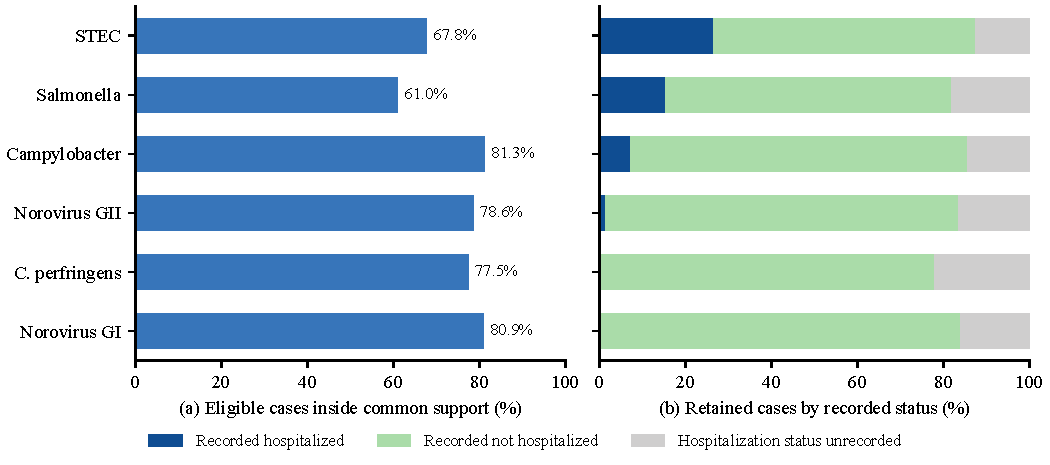
\includegraphics[width=0.92\linewidth]{figures/fig_s1_retention_recording.pdf}
  \caption{Common-support case retention and hospitalization outcome recording by pathogen group, NORS foodborne outbreaks, United States, 2009--2023. Panel (a) shows the percentage of eligible cases retained in the 12 common-support cells. Panel (b) partitions retained cases by recording status.}
  \label{fig:s-retention}
\end{figure}

\begin{figure}[!htbp]
  \centering
  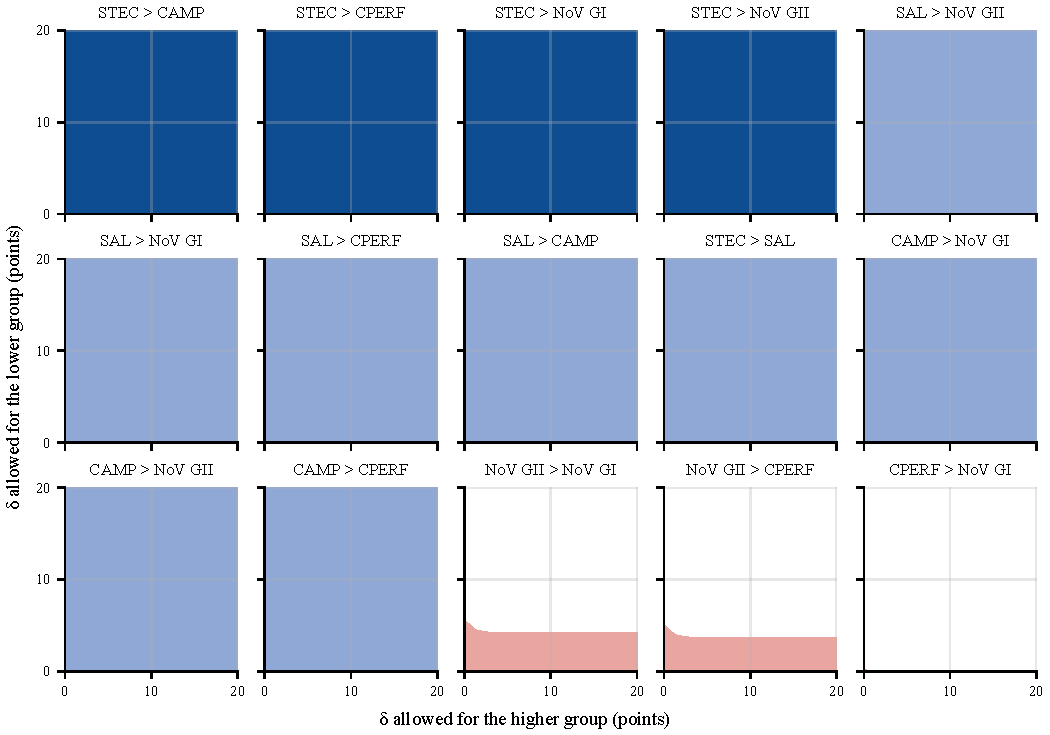
\includegraphics[width=0.95\linewidth]{figures/fig_s3_delta_2d.pdf}
  \caption{Two-dimensional tipping-point sensitivity analysis across all 15 pathogen pairs (higher group at $\delta = 0$ listed first). Shaded regions denote combinations of group-specific allowed deviations $(\delta_h, \delta_l)$ over 0--20 percentage points under which the ordering remains guaranteed; dark blue panels hold with no assumption ($\delta^{*} = \infty$).}
  \label{fig:s-delta2d}
\end{figure}

\FloatBarrier
\begin{table}[!tbp]
\centering
\scriptsize
\setlength{\tabcolsep}{3pt}
\renewcommand{\arraystretch}{1.12}
\caption{Robustness analyses, with the number of common-support cells, the number of determined pairwise orderings under worst-case bounds and at $\delta$ = 5 points, and changes relative to the main analysis.}
\label{tab:robustness}
\begin{tabular}{>{\raggedright\arraybackslash}p{1.1cm}>{\raggedright\arraybackslash}p{4.9cm}>{\raggedleft\arraybackslash}p{0.9cm}>{\raggedleft\arraybackslash}p{0.9cm}>{\raggedleft\arraybackslash}p{1.5cm}>{\raggedleft\arraybackslash}p{1.5cm}>{\raggedleft\arraybackslash}p{1.5cm}>{\raggedleft\arraybackslash}p{1.5cm}}
\toprule
Analysis & Description & Cells & Pairs & Determined, worst case & Determined, $\delta$ = 5 & Worst-case verdicts changed & $\delta$ = 0 directions changed \\
\midrule
Main & Setting $\times$ period, $\geq$ 3 outbreaks, pooled-case weights & 12 & 15 & 4 & 12 & 0 & 0 \\
R1a & Crude, no standardization, all eligible outbreaks & 1 & 15 & 5 & 12 & 1 & 1 \\
R1b & Crude within the common support (no standardization) & 1 & 15 & 4 & 13 & 0 & 0 \\
R2 & Period-only standardization (3 strata, all settings) & 3 & 15 & 5 & 12 & 1 & 1 \\
R3a & Cohort of single-etiology confirmed only & 12 & 15 & 4 & 12 & 0 & 0 \\
R3b & Cohort of records with any blank H or K dropped & 12 & 15 & 7 & 14 & 3 & 0 \\
R3c & Cohort of species-level etiology strings; records with exactly one blank outcome field dropped (3,703 outbreaks) & 11 & 15 & 4 & 12 & 0 & 0 \\
R4a & Common support $\geq$ 2 outbreaks per group per cell & 15 & 15 & 4 & 12 & 0 & 1 \\
R4b & Common support $\geq$ 5 outbreaks per group per cell & 6 & 15 & 5 & 12 & 1 & 0 \\
R5 & Drop Unknown and Multiple setting cells & 10 & 15 & 4 & 14 & 0 & 1 \\
R6a & Weights from group-balanced case mix & 12 & 15 & 4 & 12 & 0 & 0 \\
R6b & Weights from pooled outbreak mix & 12 & 15 & 4 & 12 & 0 & 1 \\
R6c & Weights from uniform over cells & 12 & 15 & 4 & 12 & 0 & 0 \\
R7 & Norovirus GI+GII combined (5 groups, 10 pairs) & 12 & 10 & 3 & 9 & NA & NA \\
\bottomrule
\end{tabular}
\par\smallskip\parbox{0.97\linewidth}{\footnotesize R7 has five groups (10 pairs), so changes versus the main analysis are not defined (NA).}
\end{table}


\begin{figure}[!htbp]
  \centering
  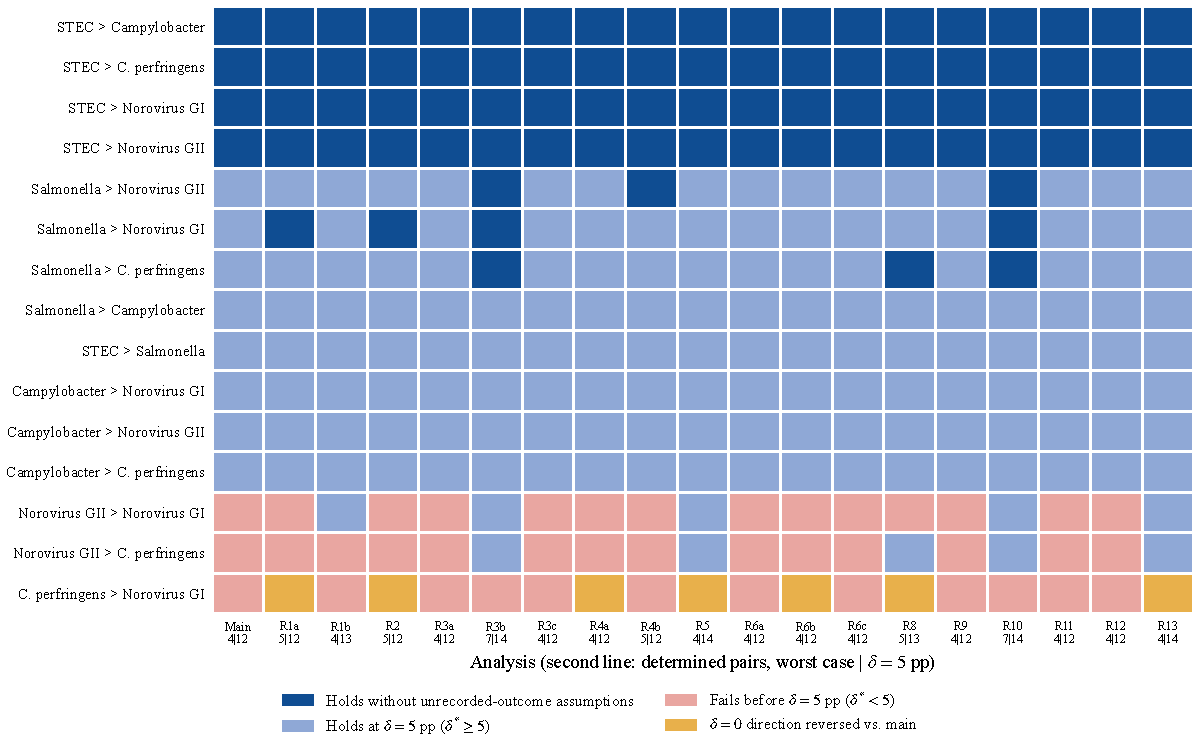
\includegraphics[width=0.95\linewidth]{figures/fig_s2_robustness.pdf}
  \caption{Pairwise ordering verdicts across the main analysis and 12 six-group robustness specifications (columns R1a--R6c; descriptions and combined norovirus variant R7 in Table~\ref{tab:robustness}). Numbers beneath each column code indicate determined pairs under worst-case bounds and at $\delta = 5$ percentage points.}
  \label{fig:s-robust}
\end{figure}

\FloatBarrier
\begin{table}[!tbp]
\centering
\scriptsize
\setlength{\tabcolsep}{3pt}
\renewcommand{\arraystretch}{1.12}
\caption{Outbreak-level bootstrap (2,000 replicates, seed 20261125; 88/2,000 resamples had $\geq$1 stratum lacking K\_rec, 0 degenerate SE entries in studentized bootstrap-t), reporting two-decimal verdict frequencies and $\delta^{*}$ percentile intervals.}
\label{tab:bootstrap}
\begin{tabular}{>{\raggedright\arraybackslash}p{2.6cm}>{\raggedleft\arraybackslash}p{2.0cm}>{\raggedleft\arraybackslash}p{2.2cm}>{\raggedleft\arraybackslash}p{2.0cm}>{\raggedleft\arraybackslash}p{2.0cm}>{\raggedleft\arraybackslash}p{2.6cm}}
\toprule
Ordering at $\delta$ = 0 & Same $\delta$ = 0 direction (\%) & Worst case, higher $>$ lower (\%) & Worst case, undetermined (\%) & Determined at $\delta$ = 5 pp (\%) & $\delta^{*}$ 2.5th--97.5th percentile (pp) \\
\midrule
STEC $>$ CAMP & 100.00 & 97.05 & 2.95 & 100.00 & 90.0--$\infty$ \\
STEC $>$ CPERF & 100.00 & 91.60 & 8.40 & 100.00 & 87.8--$\infty$ \\
STEC $>$ NoV GI & 100.00 & 93.60 & 6.40 & 100.00 & 89.6--$\infty$ \\
STEC $>$ NoV GII & 100.00 & 99.95 & 0.05 & 100.00 & $\infty$--$\infty$ \\
SAL $>$ NoV GII & 100.00 & 14.25 & 85.75 & 100.00 & 64.2--$\infty$ \\
SAL $>$ NoV GI & 100.00 & 14.55 & 85.45 & 100.00 & 47.2--$\infty$ \\
SAL $>$ CPERF & 100.00 & 24.80 & 75.20 & 100.00 & 49.6--$\infty$ \\
SAL $>$ CAMP & 100.00 & 4.20 & 95.80 & 100.00 & 23.3--$\infty$ \\
STEC $>$ SAL & 100.00 & 0.60 & 99.40 & 100.00 & 24.8--71.1 \\
CAMP $>$ NoV GI & 100.00 & 0.15 & 99.85 & 98.40 & 8.4--67.9 \\
CAMP $>$ NoV GII & 100.00 & 0.00 & 100.00 & 100.00 & 27.1--59.3 \\
CAMP $>$ CPERF & 100.00 & 1.85 & 98.15 & 100.00 & 23.7--92.5 \\
NoV GII $>$ NoV GI & 95.60 & 0.00 & 100.00 & 35.20 & 0.0--8.2 \\
NoV GII $>$ CPERF & 100.00 & 0.00 & 100.00 & 33.05 & 1.3--10.7 \\
CPERF $>$ NoV GI & 60.20 & 0.00 & 100.00 & 0.05 & 0.0--2.6 \\
\bottomrule
\end{tabular}
\end{table}

\begin{table}[!tbp]
\centering
\scriptsize
\setlength{\tabcolsep}{2.1pt}
\renewcommand{\arraystretch}{1.12}
\caption{Outbreak-cluster concentration, Multistate unrecorded case share, and standard errors across HC0, HC1, bootstrap SD (2,000 replicates), and 53 exposure-state clusters.}
\label{tab:cluster_diag}
\begin{tabular}{>{\raggedright\arraybackslash}p{1.85cm}>{\raggedleft\arraybackslash}p{1.75cm}>{\raggedleft\arraybackslash}p{2.05cm}>{\raggedleft\arraybackslash}p{1.55cm}>{\raggedleft\arraybackslash}p{3.4cm}>{\raggedleft\arraybackslash}p{3.4cm}}
\toprule
Group & Min/Med/Max n & Max HHI (min N\_eff) & Multistate unrec (\%) & SE(L) HC0/HC1/Boot/St (pp) & SE(U) HC0/HC1/Boot/St (pp) \\
\midrule
STEC & 3/22/40 & 0.479 (2.09) & 84.8 & 1.54/1.63/1.82/1.23 & 2.17/2.26/2.47/5.48 \\
Salmonella & 31/85/274 & 0.133 (7.49) & 52.8 & 0.65/0.66/0.67/1.10 & 1.96/1.98/1.88/4.83 \\
Campylobacter & 3/18/45 & 0.491 (2.04) & 0.8 & 0.81/0.84/0.87/0.88 & 2.63/2.75/2.66/2.20 \\
Norovirus GII & 16/30/301 & 0.218 (4.58) & 1.5 & 0.14/0.14/0.14/0.13 & 2.07/2.10/2.04/2.24 \\
C. perfringens & 4/10/32 & 0.501 (2.00) & 0.0 & 0.14/0.15/0.18/0.13 & 4.09/4.33/4.93/4.35 \\
Norovirus GI & 3/9/66 & 0.508 (1.97) & 5.0 & 0.10/0.11/0.11/0.13 & 3.73/3.97/3.86/3.51 \\
\bottomrule
\end{tabular}
\par\smallskip\parbox{0.97\linewidth}{\footnotesize MNW (2023) score leverage across 53 exposure-state clusters: max share = 48.3\% (worst case) and 66.8\% ($\delta$ = 5 pp) in Multistate; G\_eff = 4.04 / 2.21. Treating 219 Multistate outbreaks as singletons (271 clusters) or clustering inside 52 single states (R11) yields 0 / 0 worst-case and 12 / 12 $\delta$ = 5 significant pairs.}
\end{table}

\begin{table}[!tbp]
\centering
\scriptsize
\setlength{\tabcolsep}{3pt}
\renewcommand{\arraystretch}{1.12}
\caption{Undetermined pairs under worst-case bounds and top unrecorded-status width contributors.}
\label{tab:width}
\begin{tabular}{>{\raggedright\arraybackslash}p{2.6cm}>{\raggedleft\arraybackslash}p{1.6cm}>{\raggedright\arraybackslash}p{10.6cm}}
\toprule
Ordering at $\delta$ = 0 & Worst-case overlap (pp) & Largest contributions to interval width (group, cell, pp) \\
\midrule
SAL $>$ NoV GII & 2.7 & SAL Other | 2009-2013 (3.0); NoV GII Restaurant | 2014-2018 (2.5); NoV GII Other | 2009-2013 (2.4) \\
SAL $>$ NoV GI & 4.2 & NoV GI Unknown | 2009-2013 (4.4); NoV GI Restaurant | 2009-2013 (3.3); SAL Other | 2009-2013 (3.0) \\
SAL $>$ CPERF & 5.2 & CPERF Unknown | 2009-2013 (5.2); CPERF Other | 2009-2013 (3.0); SAL Other | 2009-2013 (3.0) \\
SAL $>$ CAMP & 4.7 & SAL Other | 2009-2013 (3.0); SAL Restaurant | 2009-2013 (2.3); CAMP Unknown | 2009-2013 (2.3) \\
STEC $>$ SAL & 7.0 & SAL Other | 2009-2013 (3.0); STEC Unknown | 2009-2013 (2.5); SAL Restaurant | 2009-2013 (2.3) \\
CAMP $>$ NoV GI & 11.2 & NoV GI Unknown | 2009-2013 (4.4); NoV GI Restaurant | 2009-2013 (3.3); NoV GI Restaurant | 2014-2018 (2.3) \\
CAMP $>$ NoV GII & 9.7 & NoV GII Restaurant | 2014-2018 (2.5); NoV GII Other | 2009-2013 (2.4); NoV GII Restaurant | 2009-2013 (2.3) \\
CAMP $>$ CPERF & 12.2 & CPERF Unknown | 2009-2013 (5.2); CPERF Other | 2009-2013 (3.0); CPERF Private home | 2009-2013 (2.7) \\
NoV GII $>$ NoV GI & 17.4 & NoV GI Unknown | 2009-2013 (4.4); NoV GI Restaurant | 2009-2013 (3.3); NoV GII Restaurant | 2014-2018 (2.5) \\
NoV GII $>$ CPERF & 18.4 & CPERF Unknown | 2009-2013 (5.2); CPERF Other | 2009-2013 (3.0); CPERF Private home | 2009-2013 (2.7) \\
CPERF $>$ NoV GI & 18.3 & CPERF Unknown | 2009-2013 (5.2); NoV GI Unknown | 2009-2013 (4.4); NoV GI Restaurant | 2009-2013 (3.3) \\
\bottomrule
\end{tabular}
\end{table}

\begin{table}[!tbp]
\centering
\scriptsize
\setlength{\tabcolsep}{3pt}
\renewcommand{\arraystretch}{1.12}
\caption{Retrospective masking experiment across 200 Monte Carlo trials on all 2,414 complete-status outbreaks (45,249 cases) in the common support. Values are means (SD) across trials by follow-up case budget.}
\label{tab:voi_masking}
\begin{tabular}{>{\raggedleft\arraybackslash}p{1.6cm}>{\raggedright\arraybackslash}p{4.2cm}>{\raggedleft\arraybackslash}p{2.4cm}>{\raggedleft\arraybackslash}p{2.4cm}>{\raggedleft\arraybackslash}p{2.4cm}}
\toprule
Budget (cases) & Policy & Worst-case det (/15) & $\delta$ = 5 det (/15) & Total overlap (pp) \\
\midrule
0 & Random follow-up & 1.57 (1.17) & 12.40 (0.59) & 171.1 (38.4) \\
0 & Largest outbreaks first & 1.57 (1.17) & 12.40 (0.59) & 171.1 (38.4) \\
0 & Width reduction greedy & 1.57 (1.17) & 12.40 (0.59) & 171.1 (38.4) \\
0 & VoI disambiguation (proposed) & 1.57 (1.17) & 12.40 (0.59) & 171.1 (38.4) \\
250 & Random follow-up & 1.78 (1.22) & 12.44 (0.61) & 164.6 (38.1) \\
250 & Largest outbreaks first & 1.58 (1.19) & 12.40 (0.59) & 170.9 (38.5) \\
250 & Width reduction greedy & 3.43 (1.07) & 12.62 (0.68) & 129.6 (31.2) \\
250 & VoI disambiguation (proposed) & 3.49 (1.25) & 12.90 (0.75) & 122.7 (32.5) \\
500 & Random follow-up & 2.06 (1.24) & 12.53 (0.62) & 156.8 (37.5) \\
500 & Largest outbreaks first & 1.68 (1.23) & 12.43 (0.61) & 167.9 (38.9) \\
500 & Width reduction greedy & 4.20 (1.08) & 12.97 (0.77) & 105.6 (26.6) \\
500 & VoI disambiguation (proposed) & 4.51 (1.32) & 13.20 (0.77) & 102.5 (30.0) \\
1,000 & Random follow-up & 2.50 (1.24) & 12.64 (0.68) & 143.2 (36.2) \\
1,000 & Largest outbreaks first & 2.01 (1.26) & 12.57 (0.66) & 152.3 (34.0) \\
1,000 & Width reduction greedy & 6.22 (1.53) & 13.43 (0.69) & 79.0 (23.9) \\
1,000 & VoI disambiguation (proposed) & 6.31 (1.61) & 13.59 (0.59) & 75.6 (24.6) \\
1,500 & Random follow-up & 2.91 (1.17) & 12.80 (0.70) & 130.2 (34.0) \\
1,500 & Largest outbreaks first & 2.29 (1.26) & 12.73 (0.73) & 141.1 (33.3) \\
1,500 & Width reduction greedy & 8.00 (1.37) & 13.96 (0.61) & 55.5 (18.4) \\
1,500 & VoI disambiguation (proposed) & 7.92 (1.63) & 13.99 (0.67) & 57.3 (19.7) \\
2,000 & Random follow-up & 3.33 (1.15) & 12.94 (0.73) & 117.7 (32.6) \\
2,000 & Largest outbreaks first & 2.69 (1.34) & 12.89 (0.74) & 128.9 (32.7) \\
2,000 & Width reduction greedy & 9.11 (1.18) & 14.29 (0.64) & 43.6 (15.8) \\
2,000 & VoI disambiguation (proposed) & 9.36 (1.65) & 14.35 (0.66) & 44.2 (15.8) \\
3,500 & Random follow-up & 4.71 (1.28) & 13.41 (0.67) & 83.6 (29.4) \\
3,500 & Largest outbreaks first & 4.03 (1.34) & 13.44 (0.67) & 91.7 (28.5) \\
3,500 & Width reduction greedy & 11.79 (0.67) & 14.91 (0.28) & 23.5 (7.7) \\
3,500 & VoI disambiguation (proposed) & 11.70 (0.96) & 14.88 (0.34) & 20.4 (8.3) \\
5,000 & Random follow-up & 6.74 (1.71) & 13.77 (0.42) & 52.2 (22.7) \\
5,000 & Largest outbreaks first & 5.95 (1.60) & 13.88 (0.36) & 56.7 (22.3) \\
5,000 & Width reduction greedy & 12.80 (0.57) & 15.00 (0.00) & 13.3 (6.1) \\
5,000 & VoI disambiguation (proposed) & 13.38 (0.81) & 14.97 (0.16) & 10.7 (4.9) \\
\bottomrule
\end{tabular}
\end{table}


\end{document}
